% !TEX TS-program = pdflatex
% !TEX encoding = UTF-8 Unicode

% This is a simple template for a LaTeX document using the "article" class.
% See "book", "report", "letter" for other types of document.

\documentclass[11pt]{article} % use larger type; default would be 10pt

\usepackage[utf8]{inputenc} % set input encoding (not needed with XeLaTeX)

%%% Examples of Article customizations

%%% PAGE DIMENSIONS
\usepackage{geometry} % to change the page dimensions
\geometry{a4paper}

\usepackage{graphicx} % support the \includegraphics command and options
\usepackage{hyperref}
\hypersetup{
  colorlinks   = true, %Colours links instead of ugly boxes
  urlcolor     = blue, %Colour for external hyperlinks
  linkcolor    = black, %Colour of internal links
  citecolor   = red %Colour of citations
}

\usepackage[parfill]{parskip} % Activate to begin paragraphs with an empty line rather than an indent

%%% PACKAGES
\usepackage{booktabs} % for much better looking tables
\usepackage{array} % for better arrays (eg matrices) in maths
\usepackage{paralist} % very flexible & customisable lists (eg. enumerate/itemize, etc.)
\usepackage{verbatim} % adds environment for commenting out blocks of text & for better verbatim
\usepackage{subfig} % make it possible to include more than one captioned figure/table in a single float
% These packages are all incorporated in the memoir class to one degree or another...
% \usepackage{hyperref}

%%% HEADERS & FOOTERS
\usepackage{fancyhdr} % This should be set AFTER setting up the page geometry
\pagestyle{fancy} % options: empty , plain , fancy
\renewcommand{\headrulewidth}{0pt} % customise the layout...
\lhead{}\chead{}\rhead{}
\lfoot{}\cfoot{\thepage}\rfoot{}

%%% SECTION TITLE APPEARANCE
\usepackage{sectsty}
% \allsectionsfont{\sffamily\mdseries\upshape} % (See the fntguide.pdf for font help)
% (This matches ConTeXt defaults)

%%% ToC (table of contents) APPEARANCE
\usepackage[nottoc,notlof,notlot]{tocbibind} % Put the bibliography in the ToC
\usepackage[titles,subfigure]{tocloft} % Alter the style of the Table of Contents
\renewcommand{\cftsecfont}{\rmfamily\mdseries\upshape}
\renewcommand{\cftsecpagefont}{\rmfamily\mdseries\upshape} % No bold!

%%% END Article customizations

%%% The "real" document content comes below...

\title{Deep Learning Lab 2018: Exercise 3}
\author{Alex Rose, Student ID 4653309}
\date{4th December, 2018} % Activate to display a given date or no date (if empty),
         % otherwise the current date is printed 

\begin{document}
\maketitle

\section{Implementation in TensorFlow}

Similar to the last exercise everything has been implemented in raw TensorFlow. See \texttt{kerosey.py} for an updated Keras-like layer API that we built, and \texttt{train\_agent.py} for the code that sets up and trains each of the models. We also used a slightly altered version of \texttt{car\_racing.py}, so that the window would fit on this laptop screen. This can be found in the Github repository at \url{https://github.com/rosea-tf/dl-lab-2018/tree/submit/}, along with the rest of our code.

Initially, we set up a model with the following architecture. Unless otherwise specified, this is what we've used in the experiments in the following sections. (Note: other basic architectures were tested ad hoc while developing code, but were found to perform worse than this one.) 

\begin{itemize}
	\item a single $96 \times 96$ grayscale input image (no history appended)
	\item two convolution operations with $3 \times 3$ kernel and 12 filters, each followed by an ELU and $2 \times 2$ MaxPool operation
	\item two fully connected layers of 256 and 128 units respectively
	\item an output layer containing five discretised actions: (do nothing, steer left, steer right, accelerate, brake)
	\item optimisation with Adam, learning rate $10^{-4}$, batch size 32, over 20 epochs (approx 11,000 minibatches)
	
\end{itemize}

Tensorboard logging was implemented in \texttt{kerosey.py}, though in practice we mostly relied on console output instead.

When testing agents on the racetrack, we seeded the Gym environment so that the same 10 episodes would be produced for each agent. Outputs of the network were also softmaxed before being translated into driving commands (so that, for example, the agent might decide to accelerate at 0.89 and steer left at 0.11: something which was not possible using the manual driving controls).

\section{Data Rebalancing}

After collecting 20,000 samples from an "expert" driver, actions were indeed found to be imbalanced: steering and braking actions were especially under-represented. We resampled the data so that actions were approximately equally frequent, and the size of the dataset was kept approximately the same (see \texttt{rebalance\_actions} in \texttt{process\_data.py}), and compared results before and after rebalancing. In both cases, training samples were also shuffled to break the correlation between successive samples, avoiding unnecessary noise in gradient descent.  The results are shown in Figure \ref{fig:balance}. For comparison, we also show our scores from driving manually.

\begin{figure}
  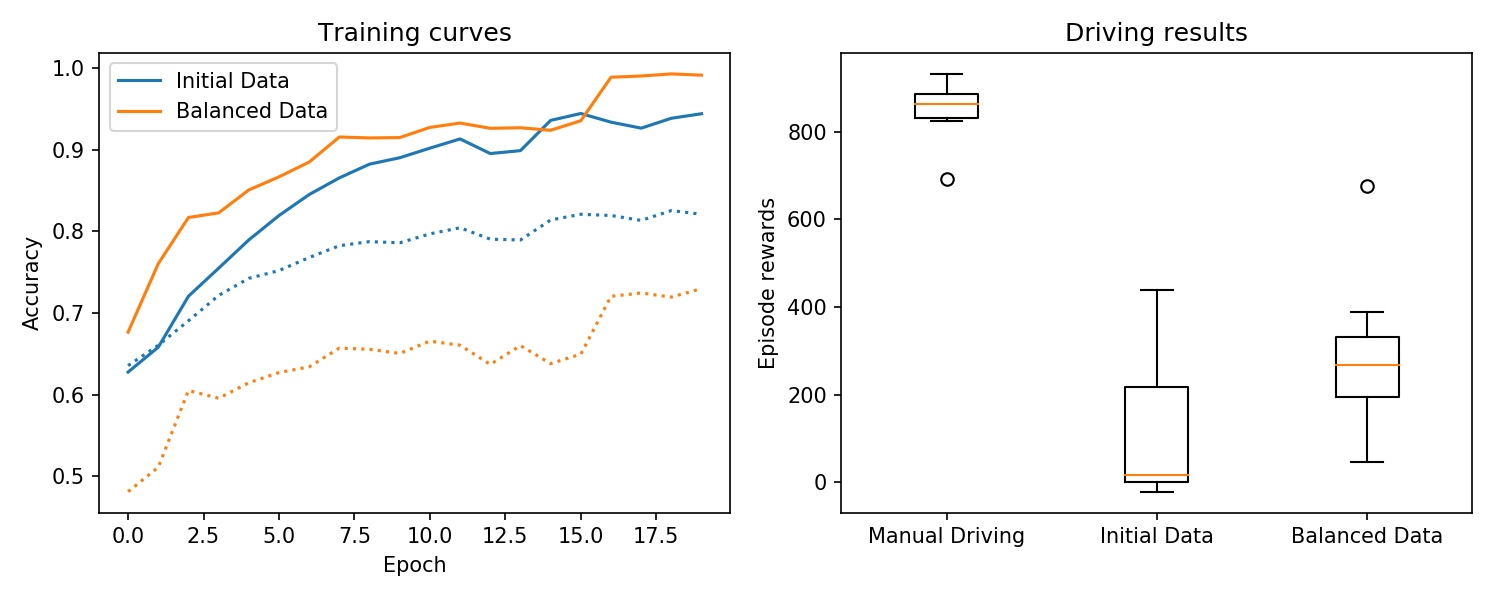
\includegraphics[width=\linewidth]{figs/balance.png}
  \caption{The effect of data augmentation \\ \textit{(Training Set: Solid, Validation Set: Dotted)}}
  \label{fig:balance}
\end{figure}

Rebalancing does not seem to improve the training curves (validation performance is actually \textit{worse!}), but it does noticeably improve performance on test episodes. Both agents show pretty awful driving (although the best result from the agent with balanced action data is about the same as our worst result from driving manually). We decide to keep our resampled data and hope it gets better.

\section{Hyperparameter Analysis: Effect of Dropout}

We analysed the effect of adding two dropout layers, one on either side of the first fully connected layer, each with the same dropout rate applied. Rates of 5\%, 10\%, and 20\% were tested. The results are shown in Figure \ref{fig:dropout}. Dropout has exactly the expected effect on training accuracy: higher rates make it worse, but there is no impact on validation accuracy. Driving results noticeably improve with 20\% dropout, though there is a lot of variance in these results. This tells us that dropout \textit{may} be partially  regularising our model and helping it generalise to new driving situations.

\begin{figure}
	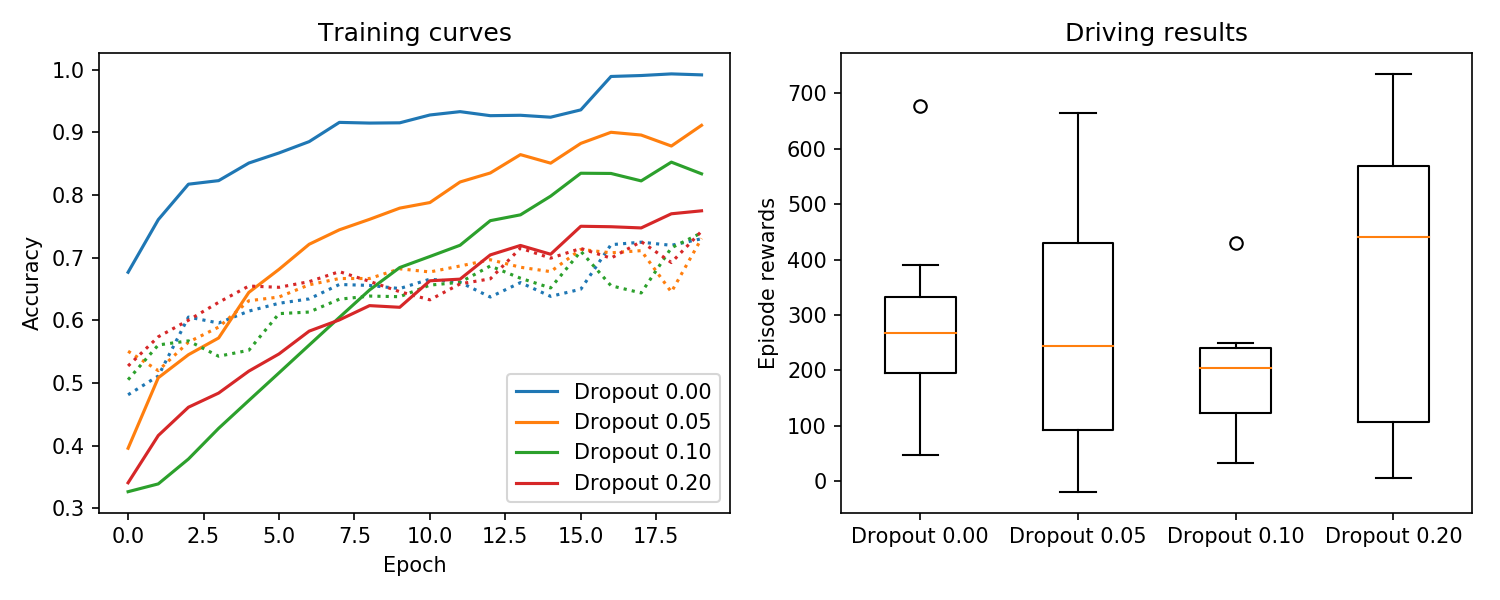
\includegraphics[width=\linewidth]{figs/dropout.png}
	\caption{The effect of dropout}
	\label{fig:dropout}
\end{figure}

\section{Effect of adding Image History}

Next, we experimented with two- and four-frame image history buffers. (Of course, these were added before the shuffling the training data.) Adding more than four images caused memory errors. We also experimented with two different architectures for processing image history:

\begin{enumerate}
	\item Adding the historical images as extra input channels in the original input image, and then processing using a set of convolution layers as normal. (Input tensor = \textit{(Batch, Width, Height, Channels [0:4])})
	\item Processing each historical image in parallel using the same set of convolution layers, with the same (shared) weights. (Input tensor = \textit{(Sequence [0:4], Batch, Width, Height, Channels [0])})
\end{enumerate}

\begin{figure}
	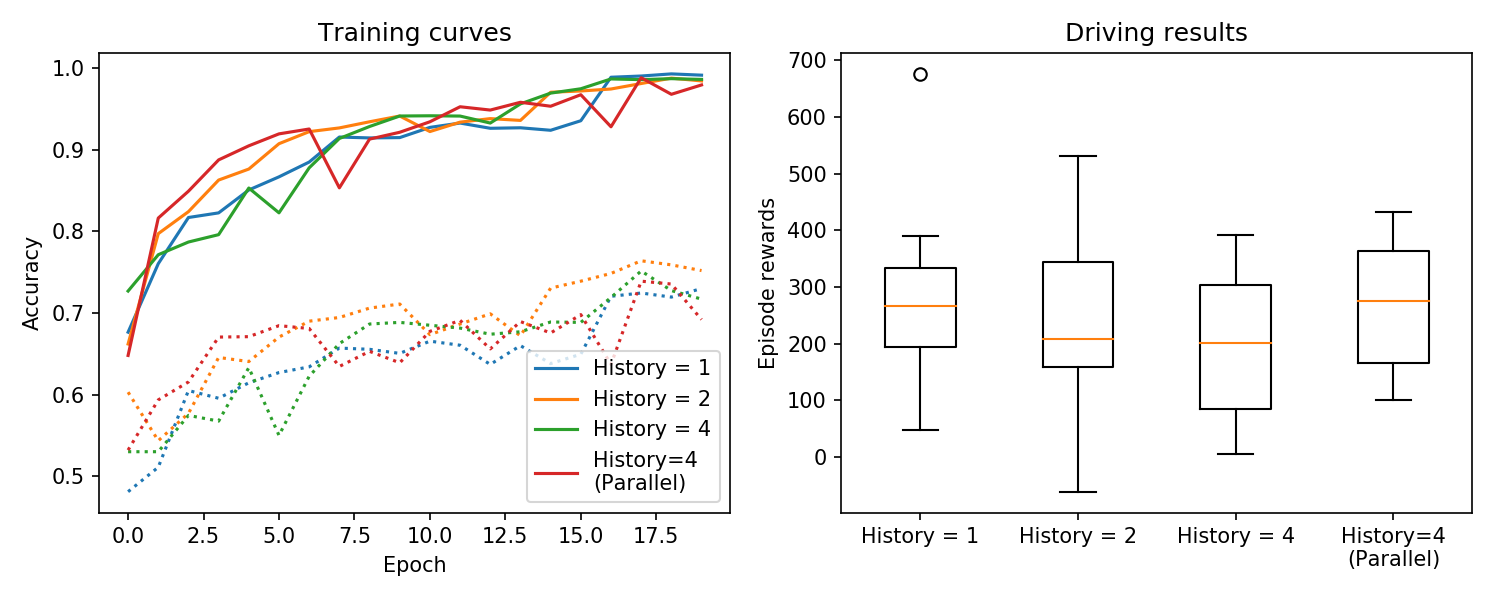
\includegraphics[width=\linewidth]{figs/history.png}
	\caption{The effect of adding historical images}
	\label{fig:history}
\end{figure}

We see in Figure \ref{fig:history} that neither method of incorporating image history into our network significantly improves results. Driving is still poor. What next?
 
\section{LSTM and BOHB: Two final desperate attempts}

First, we implemented a CNN-LSTM architecture. This was built as an extension to the "parallel" image processing described above. We flattened the output of each of the four parallel convolutions, interpreted them as a $[0,1,2,3]$ sequence, and then combined them into a 3D tensor: \textit{(Sequence, Batch, Features)}. This was then fed into an LSTM cell (again, we implemented this cell from scratch in TensorFlow), producing a \textit{(Batch, OutputFeatures)} tensor, which was then fed into the fully connected layers.

Second, we tried running a BOHB search using the HpBandSter tool developed at Freiburg (see \texttt{random\_search.py}). We used 50 iterations, and a budget range of $(3, 9)$ training epochs for each sample configuration. The best model found was then trained for 20 epochs, as with all the others tested.

Third, we tried a much higher-capacity model, using the following alterations to our basic model:

\begin{itemize}
	\item a $96 \times 96 \times 4$ grayscale historical input buffer 
	\item three convolution operations with $5 \times 5$ kernel, using 16, 32, and 64 filters respectively, each followed by an ELU and $2 \times 2$ MaxPool operation
	\item two fully connected layers of 512 and 128 units respectively
	\item dropout of 20\%
	\item (variants using LSTM and longer training were also tried, with no improvement)
\end{itemize}

\begin{figure}
	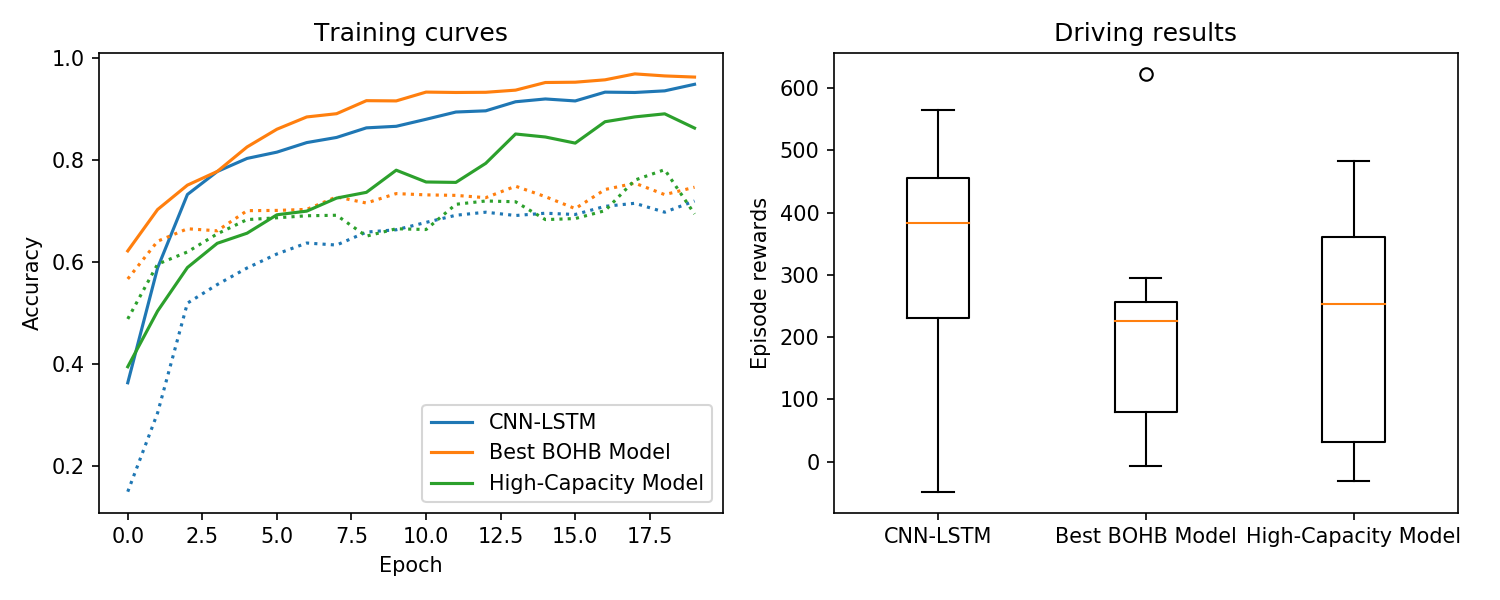
\includegraphics[width=\linewidth]{figs/final.png}
	\caption{Performance of CNN-LSTM, BOHB-optimised model, and high-capacity model}
	\label{fig:final}
\end{figure}

The results are shown in Figure \ref{fig:final}. The LSTM does show somewhat better performance than our other models, but still not exactly impressive. Hyperparameter search with BOHB was unsuccessful, and this is understandable: it evaluated the performance of configurations using validation error, and as we've seen in the figures above, validation error does a very poor job of predicting actual driving performance. Of course, evaluating with driving episode tests would have been impractical for time reasons, because of the requirement (bug?) that graphical rendering be turned on during testing. The high-capacity model was likewise unimpressive.

\section{Conclusion}

Overall, the agents we tested tend to start driving reasonably well. They can detect corners and steer properly through them. But usually on about the third or fourth corner, the agent will make a mistake, drive off the track, and never completely recover.

We might have done better with higher-quality expert data (especially with more examples of successful recovery after leaving the track), or with a different architecture, or different action encodings, or if we had not altered the zoom level on the Box2D environment. Overall, results from imitation learning were disappointing. But implementing this stuff was very interesting.

\end{document}
